\section{State-of-the-Art}\label{state-of-the-art}

\subsection{Evolution of Visualization Tools and Techniques in Healthcare}\label{evolution-of-visualization-tools-and-techniques-in-healthcare}

The evolution of visualization tools and techniques in healthcare is a testament to the field's ongoing quest to enhance the understanding and communication of complex data. The story begins with an iconic figure in healthcare history: Florence Nightingale, whose innovative work during the Crimean War laid the groundwork for modern data visualization. Nightingale's use of polar area diagrams, or coxcombs, revolutionized the way data was presented to the British parliament and played a pivotal role in reforming military and public health practices. Figure \ref{fig:coxcomb} illustrates Nightingale's visualization of mortality causes among soldiers, distinguishing deaths due to preventable diseases, wounds, and other causes through a vivid color scheme. This early example underscores the power of visualization to not only convey statistics but also to advocate for change \cite{soa7}.

\begin{figure}[ht]
  \centering
  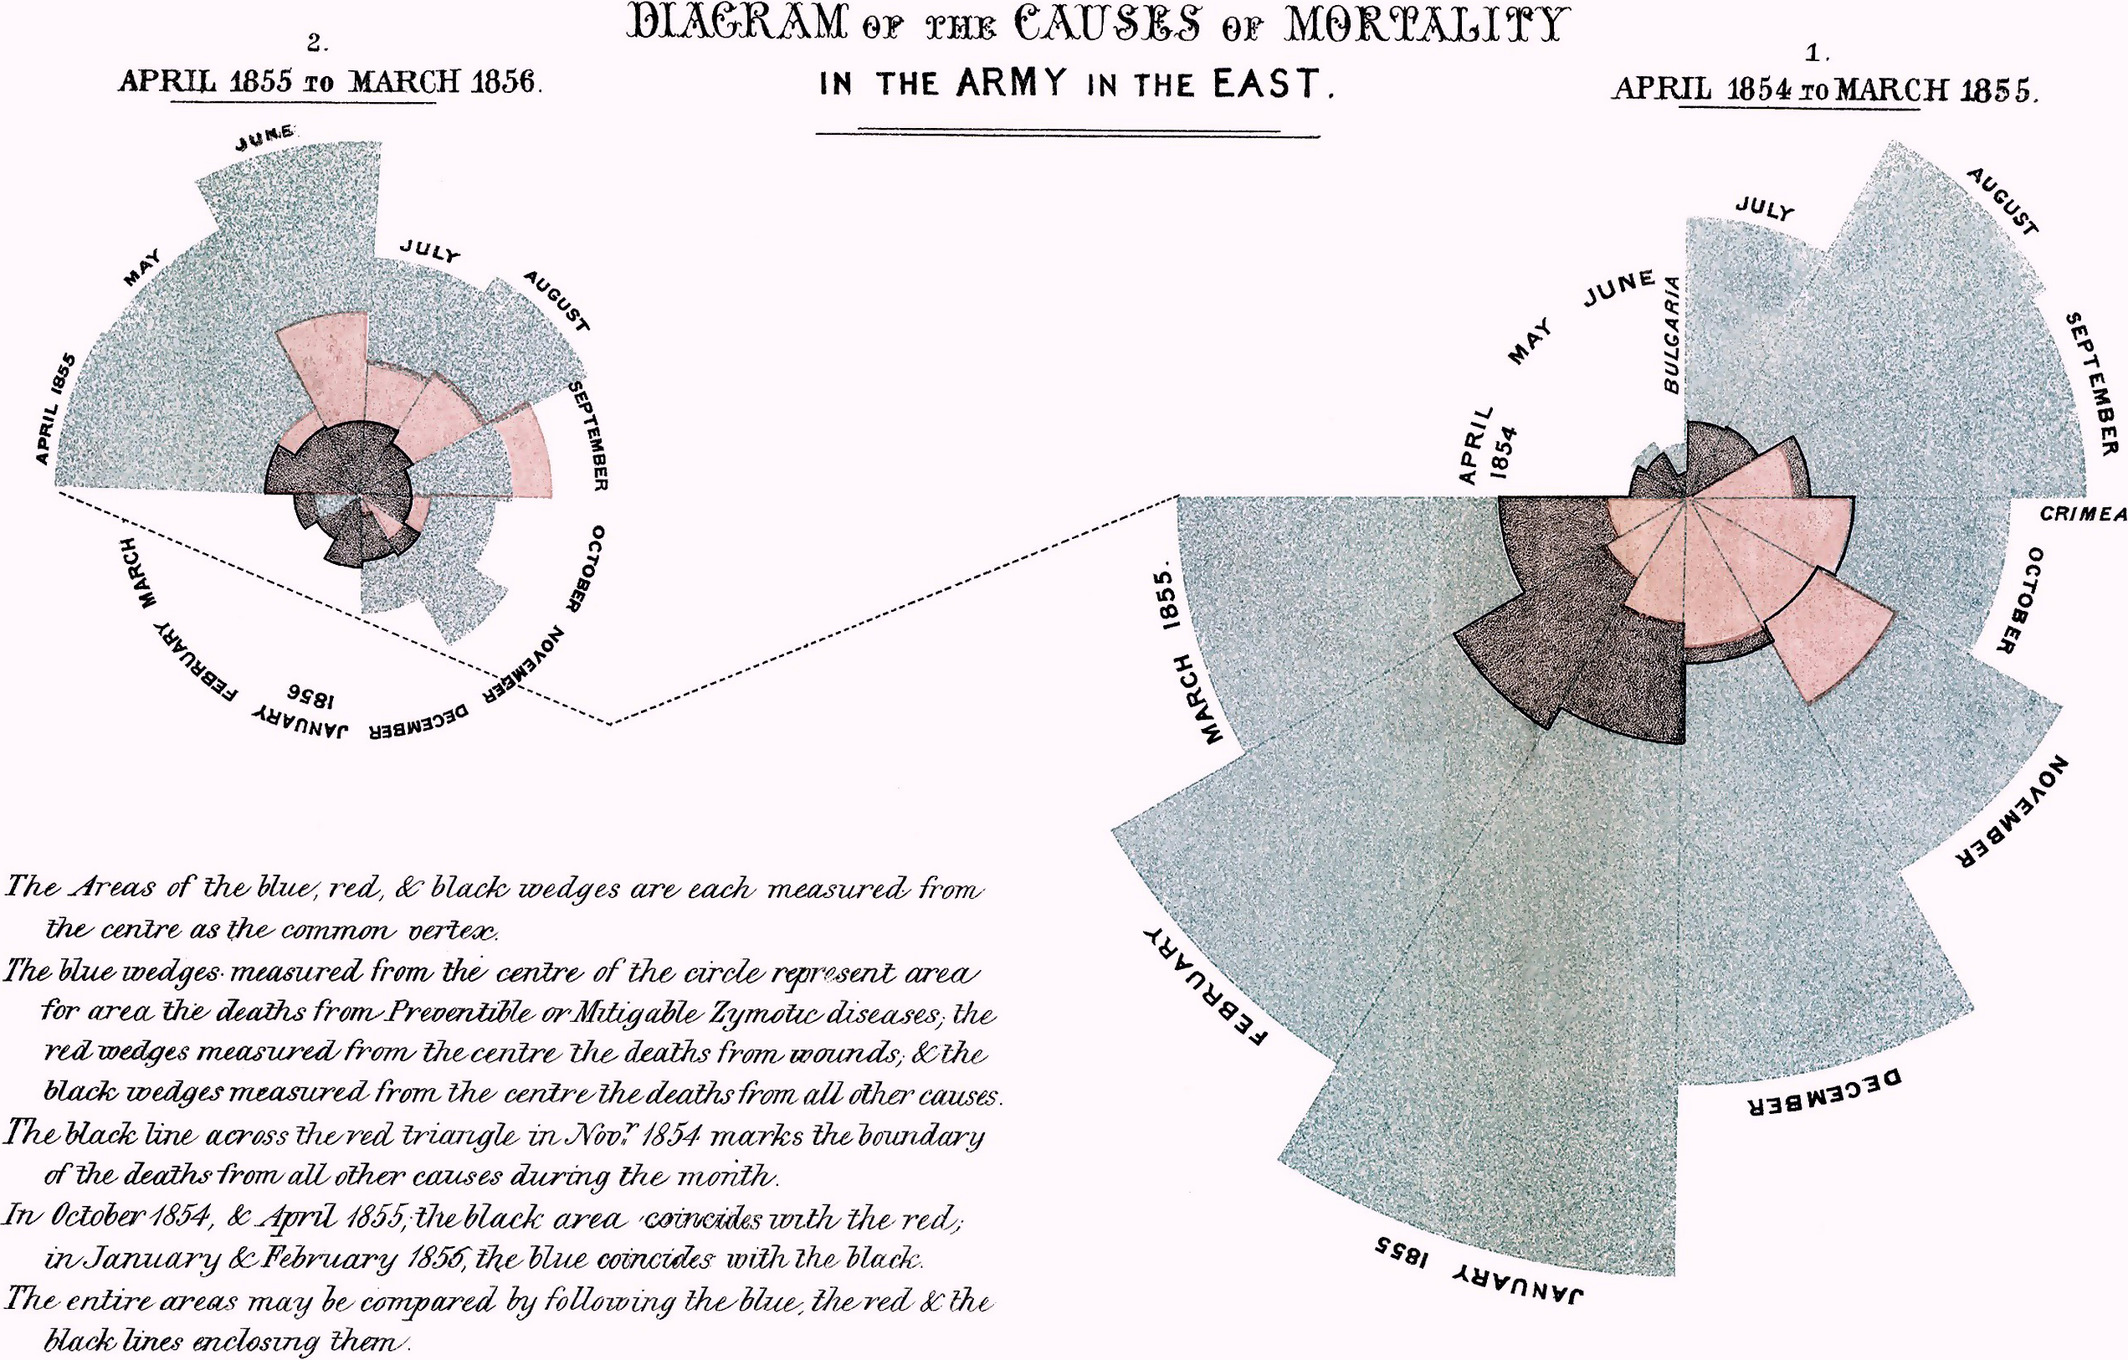
\includegraphics[width=\textwidth]{media/fig20.jpeg}
  \caption{Nightingale's coxcomb diagram on causes of mortality in the British army. Reproduced from O'connor \textit{et al} (2017)\cite{soa7}.}
  \label{fig:vsc}
\end{figure}

Today's healthcare industry, driven by data and evidence-based practice, continues to rely on the effective presentation of information. The plethora of digital health data from electronic medical records, telehealth systems, and wearable devices necessitates innovative visualization approaches to inform decisions and policies.

The science of data visualization has since matured, offering sophisticated representations of genomic, clinical, and personal health data to facilitate quick assimilation of information by diverse stakeholders.

INCLUIR CONTEÚDO INCIAL DO BACKGROUND?

\subsection{Real World Evidence}\label{real-world-evidence}

Real-World Evidence (RWE) has emerged as a significant concept in healthcare, aiming to complement and extend the insights gained from Randomized Controlled Trials (RCTs). While RCTs are the gold standard for establishing causality and assessing the efficacy of new treatments under controlled conditions, they often do not reflect the full spectrum of patient profiles encountered in routine clinical practice. RWE seeks to fill this gap by analyzing the outcomes of treatments as they are used in everyday settings, encompassing a diverse population with varying genetic backgrounds, comorbidities, and concomitant medications \cite{soa1}. This approach aims to provide a more comprehensive understanding of how treatments perform in the real world, thereby addressing the efficacy-effectiveness gap noted by Eichler \textit{et al} (2017)\cite{soa2}.

Given the intricate nature of RWE and its divergence from the more controlled environment of RCTs, transparency in methodology and findings becomes paramount. RWE studies, by capturing a diverse array of patient experiences in routine clinical settings, bring forth a complex interplay of genetic backgrounds, comorbidities, and treatments. This diversity, while enriching the data, introduces challenges in statistical evaluation due to the presence of confounding factors and biases, necessitating sophisticated analysis techniques for accurate interpretation \cite{soa3}\cite{soa4}.

The need for transparency extends to the sharing of data and code, facilitating computational reproduction and peer validation. However, the use of routinely collected electronic healthcare data often restricts public sharing due to privacy and regulatory constraints. This limitation underscores the importance of detailed reporting in RWE studies, providing a clear and comprehensive account of methodologies, data handling, and analytical strategies employed. Such detailed documentation ensures that, even when data cannot be shared, the processes and conclusions remain open to scrutiny and understanding. \cite{soa5}\cite{soa6}.

Wang et al. (2021) advocate for the harmonization and standardization of RWE practices to foster reproducibility and reliability in the field. This includes developing templates for planning and reporting that reduce inconsistencies and elevate the quality of RWE research. By adhering to these structured approaches and emphasizing transparency, the field of RWE can continue to provide valuable, nuanced insights into healthcare practices and outcomes, bridging the gap between clinical research and everyday medical care. The complexity of RWE findings necessitates not just textual explanation but also extensive visualizations. These visual tools are essential for illustrating the nuances of sub-analyses, sensitivity analyses, and other supplementary investigations, often accumulating into a substantial part of the supplementary material. Through detailed tables, figures, and a multitude of visual representations, researchers can offer a more transparent and digestible overview of their findings, aiding in the comprehension and further investigation of the intricate data landscapes characteristic of RWE studies \cite{soa5}.

\subsection{Visualization for Electronic Health Records (EHR)}\label{visualization-for-electronic-health-records-ehr}

The paper "EHR STAR: The State-Of-the-Art in Interactive EHR Visualization" provides an up-to-date overview of the state-of-the-art in Electronic Health Record (EHR) visualization. It presents a comprehensive analysis of the literature and open access healthcare data sources related to EHR visualization, emphasizing the importance of this topic. The paper refers to the significance of EHRs in modern medicine, positioning them as a standard practice and highlighting the potential for innovative visual methods to support clinical decision-making and research. The poor usability of EHRs is also noted, with international publications reporting no significant improvements over time. The significance of interactive visualization applications that interface seamlessly with EHR systems is highlighted, particularly in facilitating dynamic exploration and rapid extraction of patient data for researchers \cite{soa8}.

The EHR STAR project has developed an interactive EHR STAR Browser, which serves as a comprehensive platform containing relevant literature described in the corresponding review. This browser provides a user-friendly interface for accessing and visualizing EHR data, supporting dynamic exploration and rapid extraction of patient data for researchers \cite{soa8}.



\subsection{Research Oriented Visualizations}\label{research-oriented-visualizations}

The focus of research primarily on EHR visualization within clinical interfaces has highlighted the need for visual tools that support clinical decisions. However, the development of visualizations dedicated to research purposes has been less prominent. This gap suggests an opportunity for further innovation and implementation of visualization tools tailored for research, potentially enhancing the efficiency and efficacy of healthcare data analysis.

\subsection{Advances in Interactive and Real-Time Visualization}\label{advances-in-interactive-and-real-time-visualization}

\subsection{Challenges in Healthcare Data Visualization}\label{challenges-in-healthcare-data-visualization}

Healthcare data visualization is an evolving discipline that faces a multitude of challenges, exacerbated by the field's inherent complexity and rapid technological advancements. These challenges, ranging from data diversity to security concerns, substantially impact the effectiveness and adoption of visualization tools in healthcare settings. Table \ref{tab:healthcare-challenges} summarizes these critical issues, providing an overview of the hurdles that need to be navigated. This subsection will detail each of these topics, shedding light on the specific nature of the challenges and their implications for healthcare data visualization.

\begin{table}[ht]
\caption{Summary of Challenges in Healthcare Data Visualization}
\label{tab:healthcare-challenges}
\centering
\begin{tabular}{|p{0.2\linewidth}|p{0.5\linewidth}|p{0.2\linewidth}|}
\hline
\textbf{Challenge} & \textbf{Description} & \textbf{References} \\ \hline
Multidisciplinary Research Themes & Need for expertise in multiple domains such as visualization, NLP, and ML, making scope definition and organization challenging. & \cite{soa9} \\ \hline
Data Protection Laws & Stringent requirements of GDPR and HITECH significantly complicate data acquisition and navigating legal and ethical constraints. & \cite{soa11, soa10} \\ \hline
Accessibility of Open Datasets & Privacy concerns limit the availability of open datasets crucial for developing and refining visualization tools. & \cite{soa9} \\ \hline
Necessity for Customized Visualization Tools & Requirement to work with processed data or aggregate parameters demands highly customizable visualization tools. & \cite{soa12, soa13} \\ \hline
Data Heterogeneity and High-Dimensionality & Varied and complex nature of healthcare data makes standard visualization tools insufficient. & \cite{soa12, soa13} \\ \hline
Resistance to Adoption & Resistance from clinical professionals due to lack of expertise in complex computer systems, including visualization tools. & \cite{soa14} \\ \hline
Bureaucratic Barriers to Data Access & Time-consuming registration and verification processes hinder efficient data utilization. & \cite{soa15} \\ \hline
Data Interoperability & Absence of uniform health data standards prevents seamless data exchange and integration across systems. & \cite{soc21} \\ \hline
Big Data Challenges & Traditional visualization methods struggle to handle the volume, variety, and velocity of big healthcare data. & \cite{soa13} \\ \hline
Visual Analytics Development & Lack of understanding and availability of advanced methods to address complex questions limits progress in visual analytics. & \cite{soa17, soa18} \\ \hline
Information Overload & Risk of ignoring or misinterpreting crucial data due to overwhelming quantity and complexity of information. & \cite{soa19, soa20} \\ \hline
\end{tabular}
\end{table}


One of the inherent is the multidisciplinary nature of the research themes involved. Projects often require expertise in visualization, Natural Language Processing (NLP), and Machine Learning (ML), making it difficult to establish a well-defined classification and scope to organize the previous knowledge effectively \cite{soa9}.

The sensitive nature of electronic healthcare data adds another layer of complexity, necessitating strict adherence to data protection laws such as GDPR \cite{soa11} in Europe and HITECH \cite{soa10} in the United States of America. This legal and ethical landscape can significantly complicate data acquisition for research, often requiring researchers and institutions to navigate a maze of regulatory requirements \cite{soa9}.

Open datasets, which are a cornerstone for developing and refining visualization tools, often become less accessible due to these privacy concerns. As a result, researchers seeking to improve visualizations are frequently unable to access the breadth of raw data required to create comprehensive and detailed visual representations. The scarcity of readily available datasets hampers the development of new and innovative visualization techniques that could otherwise enhance the understanding and communication of complex healthcare information \cite{soa9}.

Moreover, when visualizations are necessary, they may have to be constructed from data that has already undergone extensive processing. Researchers are sometimes left to work with aggregate parameters, such as model weights or summary statistics, rather than the raw data itself. This creates a unique demand for specialized visualization tools that can operate with processed data or aggregate parameters in reports, unlike other fields where observation-level data may be more readily accessible,

The diverse and intricate nature of healthcare data presents a notable challenge for visualization tools. A typical dataset might blend various data types—free text from clinical notes, numerical values from lab tests, ordinal scales from surveys, images from radiology, and categorical codes from diagnoses. When combined with the high-dimensional nature of such data, this can overwhelm standard visualization tools, which may lack the flexibility to handle such complexity effectively \cite{soa12}\cite{soa13}.

Given this complexity, it's often impractical to rely on a single visualization tool to meet the diverse needs of different healthcare projects. Customization becomes key, with tools needing to be highly adaptable to accommodate the specific demands of each unique dataset and research question. This often means that tools must be tailored from the ground up, incorporating specific functionalities to accurately represent the multifaceted nature of healthcare data.
As explained before, visualization tools must operate on aggregate data or summary reports rather than raw data. These reports often deviate from standard tabular formats, requiring additional layers of processing to render them into coherent visual representations. The necessity to adapt to these non-standard data formats means that visualization in healthcare often demands a bespoke approach, with tools designed to interpret and display data in ways that diverge from the norm found in other sectors where data is more homogenized and less sensitive \cite{soa12}\cite{soa13}.

Resistance from clinical professionals, often stemming from a lack of expertise in complex computer systems including visualization, has been identified as a primary barrier to the adoption and deployment of EHR visualization systems within clinical environments \cite{soa14}. This resistance is compounded by the challenges researchers face in accessing EHR data due to time-consuming registration and verification processes required by some data providers \cite{soa15}. The necessity for automation becomes apparent in this context. Automated systems can streamline the data visualization process, enabling researchers to bypass the repetitive and time-consuming steps involved in data preparation and visualization.

Achieving data interoperability in healthcare is an ongoing challenge, as widespread adoption of uniform health data standards is yet to be realized. This lack of consensus on a standardized format for health data, including Electronic Health Records (EHR), impedes seamless data exchange and integration across various healthcare systems \cite{soc21}.

Moreover, traditional data visualization methods are often inadequate for handling the sheer volume of big data in healthcare. Many datasets are too large to fit into memory or are distributed across clusters, posing significant challenges to meaningful and valuable presentation \cite{soa13}. Real-time analysis of such complex data is increasingly important, and factors such as data value and veracity must be considered \cite{soa13}.

Despite the critical role of visual analytics in healthcare decision-making, a lack of understanding, availability, development, and application of methods to address complex questions remains a significant hurdle. This gap hinders the development of evidence and effective decision-making processes \cite{soa17}\cite{soa18}.

Information overload further complicates the landscape. With the abundance of variables that exceed the limits of human cognition, healthcare professionals are at risk of ignoring or misinterpreting crucial data. The problem of information overload is pervasive in healthcare, where it can lead to incorrect data interpretations, wrong diagnoses, and missed early warning signs \cite{soa19}\cite{soa20}. The multi-modal and heterogeneous properties of EHR data, along with frequent redundant, irrelevant, and subjective measures, present substantial challenges in synthesizing information to derive actionable insights \cite{soa20}.

Addressing these challenges requires an interdisciplinary approach, combining advances in computational techniques with a deep understanding of the clinical context. It also necessitates the development of new tools and methods that can handle the volume, variety, and complexity of healthcare data while ensuring that the insights derived are both accurate and actionable.

\subsubsection{Data Complexity and Heterogeneity}\label{data-complexity-and-heterogeneity}
\subsubsection{Privacy and Security in Health Data}\label{privacy-and-security-in-health-data}
\subsubsection{Scalability and Performance in Visualization Tools}\label{scalability-and-performance-in-visualization-tools}

\subsection{Comparative Analysis of Visualization Tools}\label{comparative-analysis-of-visualization-tools}
\subsubsection{Evaluation of Existing Solutions}\label{evaluation-of-existing-solutions}
\subsubsection{Gaps and Opportunities for Visual Viper}\label{gaps-and-opportunities-for-visual-viper}

\subsection{Future Directions in Healthcare Visualization}\label{future-directions-in-healthcare-visualization}
\subsubsection{Emerging Technologies and Approaches}\label{emerging-technologies-and-approaches}
\subsubsection{Anticipated Challenges and Solutions}\label{anticipated-challenges-and-solutions}
